\documentclass[12pt,a4paper]{article}

\usepackage[utf8]{inputenc}
\usepackage[T1]{fontenc}
\usepackage{mathpazo}
\usepackage[margin=1.15in]{geometry}
\usepackage{setspace}
\usepackage{hyperref}
\usepackage{titlesec}
\usepackage{amsmath,amsthm,amssymb}
\usepackage{booktabs}
\usepackage{enumitem}
\usepackage{fancyhdr}
\usepackage{xcolor}
\usepackage{tcolorbox}
\usepackage{tikz}
\usepackage{array}
\usepackage{float}

\newtcolorbox{vizpanel}[1][]{colback=gray!4, colframe=gray!50!black,
  fonttitle=\bfseries, title={Visualization: #1}, sharp corners, boxrule=0.5pt}

\hypersetup{colorlinks=true, linkcolor=blue!70!black, citecolor=black, urlcolor=blue!70!black}

\titleformat{\section}{\large\bfseries}{\thesection}{0.7em}{}
\titleformat{\subsection}{\normalsize\bfseries}{\thesubsection}{0.7em}{}
\titleformat{\subsubsection}{\normalsize\itshape}{\thesubsubsection}{0.7em}{}

\newtheorem{definition}{Definition}[section]
\newtheorem{proposition}[definition]{Proposition}
\newtheorem{theorem}[definition]{Theorem}
\newtheorem{lemma}[definition]{Lemma}
\newtheorem{corollary}[definition]{Corollary}
\newtheorem{example}[definition]{Example}
\theoremstyle{remark}
\newtheorem{remark}[definition]{Remark}

\newcommand{\R}{\mathbb{R}}
\newcommand{\ones}{\mathbf{1}}
\newcommand{\x}{\mathbf{x}}
\DeclareMathOperator*{\argmax}{arg\,max}

\newtcolorbox{intuition}[1][]{colback=blue!3, colframe=blue!40!black, fonttitle=\bfseries, title={Intuition: #1}, sharp corners, boxrule=0.5pt}
\newtcolorbox{keyinsight}[1][]{colback=orange!5, colframe=orange!60!black, fonttitle=\bfseries, title={Key Structural Insight}, sharp corners, boxrule=0.5pt}
\newtcolorbox{prebisch}[1][]{colback=green!3, colframe=green!40!black, fonttitle=\bfseries, title={Prebisch Connection: #1}, sharp corners, boxrule=0.5pt}

\setlength{\parindent}{1.5em}
\onehalfspacing
\setlength{\headheight}{14pt}
\pagestyle{fancy}
\fancyhf{}
\fancyhead[L]{\small\itshape Chapter 7: The Bargaining Equilibrium}
\fancyhead[R]{\small\thepage}
\renewcommand{\headrulewidth}{0.4pt}

\title{\vspace{-1cm}\textbf{Chapter 7} \\[0.5em]
\LARGE The Bargaining Equilibrium \\[0.3em]
\large\textit{Where Power Meets Prices}}
\author{}
\date{}

\begin{document}
\maketitle
\thispagestyle{fancy}

\begin{quote}
\textit{``El fundamento de la dependencia es la superexplotaci\'{o}n del trabajo, es decir, el hecho de que el trabajo se remunera por debajo de su valor.''}\\[0.3em]
\textnormal{[``The foundation of dependence is the superexploitation of labor --- that is, the fact that labor is remunerated below its value.'']}\\
\hfill --- Ruy Mauro Marini, \textit{Dial\'{e}ctica de la dependencia} (1973)
\end{quote}

\vspace{0.3em}

\begin{quote}
\textit{``The market gives you what you can pay for. The structure determines what you can pay.''}\\
\hfill --- Celso Furtado (paraphrased)
\end{quote}

\vspace{0.5em}

\begin{quote}
\textit{``$x_i^* = f(\boldsymbol{\pi}(W), \boldsymbol{\omega}, p)$. That is the whole chapter.''}\\
\hfill --- This book
\end{quote}

\vspace{1em}

Chapter~1 derived the competitive equilibrium: every agent maximizes utility at market prices, markets clear, and the allocation is Pareto efficient. Chapter~6 showed that this requires $\boldsymbol{\pi} = \frac{1}{N}\ones$ --- equal power. This chapter asks: what is the equilibrium when power is unequal?

The answer is the \textit{bargaining equilibrium}: a generalized Nash bargaining solution where the weights are not assumed but derived from the weight matrix $W$ through the Perron eigenvector. Power enters the allocation problem. The salte\~{n}a vendor's compadrazgo bond, the gas executive's regulatory leverage, the girl in Potos\'{i}'s information network --- all of these shape $W$, which shapes $\boldsymbol{\pi}$, which shapes the allocation.

The main results: (1)~the bargaining equilibrium exists and is unique under standard conditions; (2)~it reduces to the competitive equilibrium when $\boldsymbol{\pi} = \frac{1}{N}\ones$; (3)~the welfare loss from power asymmetry has a clean decomposition into power, externality, and interaction components; and (4)~the direction of inefficiency is determined by $\boldsymbol{\pi}$: powerful agents consume too much, powerless agents too little.


%% =====================================================================
\section{From Competitive to Bargaining}
\label{sec:from_to}
%% =====================================================================

\subsection{Why Not Walras?}

The Walrasian equilibrium assumes price-taking: every agent is so small relative to the market that she cannot affect prices. This implies equal power. But in most real economies, agents are not equal:

\begin{itemize}
\item A monopsony employer in a company town sets wages, not the market.
\item A landlord with the only irrigated field in a valley sets the sharecropping rate.
\item A country that exports 40\% of global lithium (Chile) affects the world price.
\item A platform (Amazon, Uber) sets the terms of trade for millions of small sellers.
\end{itemize}

In each case, some agent has structural power --- a position in $W$ that gives her Perron weight $\pi_i > 1/N$ --- and she uses that power to pull the allocation toward herself. The Walrasian model cannot capture this because it assumes the power away.

The bargaining equilibrium keeps everything the Walrasian model has (preferences, endowments, production) and adds one object: the power vector $\boldsymbol{\pi}(W)$.


\subsection{A Two-Person Example First}

Before the general model, let us see the mechanism in the simplest possible case.

\begin{example}[The Landlord and the Farmer]\label{ex:landlord}
Two agents: a Landlord ($L$) and a Farmer ($F$). One good (output). The Landlord owns the land ($\omega_L = 10$); the Farmer owns labor ($\omega_F = 2$). Together they can produce $Y = 20$ (more than the sum of endowments, so there are gains from cooperation). Apart, the Landlord produces 10 (land alone) and the Farmer produces 2 (labor alone).

The \textbf{surplus} from cooperation is $S = 20 - 10 - 2 = 8$. How is it divided?

\textbf{Competitive answer:} Each factor is paid its marginal product. If the production function is $Y = K^{0.5}L^{0.5}$ with $K = 10$ and $L = 2$, then $MPK = 0.5 \times 20/10 = 1$ and $MPL = 0.5 \times 20/2 = 5$. The Farmer gets $5 \times 2 = 10$ and the Landlord gets $1 \times 10 = 10$. Equal split. The Farmer's income quintuples; the Landlord's stays the same. This assumes perfect competition in both factor markets.

\textbf{Bargaining answer:} The surplus is divided according to power weights $\boldsymbol{\pi} = (\pi_L, \pi_F)$. The Nash bargaining solution gives each agent their disagreement payoff plus a share of the surplus:
\begin{equation}\label{eq:nash_two}
x_L = 10 + \pi_L \times 8 = 10 + 8\pi_L, \qquad x_F = 2 + \pi_F \times 8 = 2 + 8\pi_F.
\end{equation}

If the Landlord has more power ($\pi_L = 0.7$, $\pi_F = 0.3$): $x_L = 15.6$, $x_F = 4.4$. The Farmer's income doubles (not quintuples). The Landlord captures most of the surplus.

If the Farmer has more power ($\pi_L = 0.3$, $\pi_F = 0.7$): $x_L = 12.4$, $x_F = 7.6$. The Farmer does much better.

If power is equal ($\pi_L = \pi_F = 0.5$): $x_L = 14$, $x_F = 6$. Neither the competitive answer (10, 10) nor the equal-split-of-surplus answer (14, 6). The bargaining solution with equal power gives each agent their disagreement payoff plus half the surplus.

\begin{center}
\begin{tabular}{lccc}
\toprule
Scenario & Landlord & Farmer & Surplus share to $F$ \\
\midrule
Autarky & 10.0 & 2.0 & --- \\
Competitive (MPL pricing) & 10.0 & 10.0 & 100\% \\
Bargaining ($\pi_L = 0.7$) & 15.6 & 4.4 & 30\% \\
Bargaining ($\pi_L = 0.5$) & 14.0 & 6.0 & 50\% \\
Bargaining ($\pi_L = 0.3$) & 12.4 & 7.6 & 70\% \\
\bottomrule
\end{tabular}
\end{center}
\end{example}

\begin{intuition}[Why the competitive answer is a special case]
The competitive equilibrium gives the Farmer 100\% of the surplus --- because competitive factor markets price labor at its marginal product, which is very high when labor is scarce (only 2 units of labor with 10 units of land). But this requires the Farmer to have an outside option that credibly threatens the Landlord: if the Farmer can walk away and sell her labor elsewhere at the competitive wage, the Landlord must match that wage.

In a competitive market, the ``outside option'' is the market itself: any buyer or seller can transact with any other buyer or seller. This is $W = \frac{1}{N}\ones\ones'$ --- everyone is connected to everyone, so nobody has hold-up power.

In a real village, the Farmer's outside option may be very limited: the Landlord is the only employer within walking distance, the Farmer has no savings to relocate, and social norms (the compadrazgo bond, the patron-client relationship) create obligations that limit exit. The Farmer's position in $W$ is peripheral: $W_{FL}$ is large (the Farmer depends on the Landlord) but $W_{LF}$ is small (the Landlord can replace the Farmer). This asymmetry gives the Landlord high $\pi_L$ and allows her to capture most of the surplus.

The competitive model assumes this away. The bargaining model puts it back.
\end{intuition}


%% =====================================================================
\section{The General Bargaining Problem}
\label{sec:general}
%% =====================================================================

\subsection{Setup}

$N$ agents, $L$ goods, preferences $U_i(x_i)$ (with externalities from $W^U$ as in Chapter~5), endowments $\boldsymbol{\omega} = (\omega_1, \ldots, \omega_N)$, and a composite weight matrix $W$ with Perron eigenvector $\boldsymbol{\pi} = (\pi_1, \ldots, \pi_N)'$.

Each agent's \textbf{disagreement utility} --- what she gets if bargaining fails and she consumes her endowment --- is:
\begin{equation}\label{eq:disagreement}
d_i = V_i(\boldsymbol{\omega}) = U_i(\omega_i) + \gamma_U \sum_{j \neq i} W^U_{ij} U_j(\omega_j).
\end{equation}

The \textbf{surplus} for agent $i$ from any allocation $\x = (x_1, \ldots, x_N)$ is:
\begin{equation}
S_i(\x) = V_i(\x) - d_i.
\end{equation}

\begin{definition}[The Bargaining Equilibrium]\label{def:bargaining_eq}
The \textbf{bargaining equilibrium} is the allocation $\x^*$ that solves:
\begin{equation}\label{eq:bargaining}
\max_{\x \geq 0} \sum_{i=1}^N \pi_i \ln S_i(\x) \qquad \text{subject to} \qquad \sum_{i=1}^N x_{i\ell} = \bar{\omega}_\ell, \quad \ell = 1, \ldots, L,
\end{equation}
where $\boldsymbol{\pi} = \boldsymbol{\pi}(W)$ is the left Perron eigenvector of the composite weight matrix, and feasibility requires total consumption equals total endowment for each good.
\end{definition}

\begin{intuition}[What the bargaining problem maximizes]
The objective~\eqref{eq:bargaining} is the \textbf{weighted Nash product}: the weighted sum of log-surpluses. Each agent's log-surplus $\ln S_i$ is weighted by her power $\pi_i$. An agent with higher power has more ``voting weight'' in the allocation decision --- her surplus matters more.

When $\boldsymbol{\pi} = \frac{1}{N}\ones$ (equal power), this is the standard symmetric Nash bargaining solution. When $\pi_i$ varies, it is the asymmetric Nash bargaining solution with weights determined by the network.

Why logarithms? The Nash axioms (invariance to affine utility transformations, Pareto efficiency, symmetry, independence of irrelevant alternatives) characterize the product $\prod_i S_i^{\pi_i}$ as the unique solution satisfying these properties. Taking logs converts the product to a sum, making the optimization problem concave.
\end{intuition}


\subsection{First-Order Conditions}

For the case without utility externalities ($\gamma_U = 0$, so $V_i = U_i$ and $S_i = U_i(x_i) - U_i(\omega_i)$), the Lagrangian is:
\begin{equation}
\mathcal{L} = \sum_{i=1}^N \pi_i \ln\bigl(U_i(x_i) - U_i(\omega_i)\bigr) - \sum_{\ell=1}^L \mu_\ell \left(\sum_i x_{i\ell} - \bar{\omega}_\ell\right).
\end{equation}

The first-order condition for $x_{i\ell}$ is:
\begin{equation}\label{eq:foc_bargaining}
\frac{\pi_i}{S_i(\x^*)} \cdot \frac{\partial U_i}{\partial x_{i\ell}} = \mu_\ell, \qquad \forall \, i, \ell.
\end{equation}

\begin{intuition}[Reading the FOC]
The left side is the ``power-adjusted marginal utility'': agent $i$'s marginal utility of good $\ell$, scaled by her power-to-surplus ratio $\pi_i / S_i$. At the optimum, this must be equal across all agents for each good.

Compare with the competitive FOC: $\frac{\partial U_i}{\partial x_{i\ell}} / \lambda_i = p_\ell$, where $\lambda_i$ is agent $i$'s marginal utility of wealth. In the competitive case, the shadow price $\mu_\ell$ equals the market price $p_\ell$, and the right-hand side is the same for everyone. In the bargaining case, the shadow price $\mu_\ell$ is still equalized across agents, but the left side carries the extra term $\pi_i / S_i$: power matters.

An agent with high $\pi_i$ relative to $S_i$ (powerful but not yet receiving much surplus) gets a higher marginal weight --- the solution gives her more. An agent with low $\pi_i$ (powerless) gets less, even if her marginal utility is high. This is the mechanism of structural inequality.
\end{intuition}


\subsection{The Bargaining Allocation with LQ Utility}

To build full intuition, we solve the model explicitly for linear-quadratic utility.

\begin{example}[The LQ Bargaining Equilibrium]\label{ex:LQ_bargaining}
$N$ agents, one good, $U_i(x_i) = x_i - \frac{\kappa}{2}x_i^2$, total endowment $\Omega$, endowments $\boldsymbol{\omega}$, power $\boldsymbol{\pi}$.

The surplus is $S_i = U_i(x_i) - U_i(\omega_i) = (x_i - \omega_i) - \frac{\kappa}{2}(x_i^2 - \omega_i^2) = (x_i - \omega_i)(1 - \frac{\kappa}{2}(x_i + \omega_i))$.

For small trades ($x_i \approx \omega_i$), $S_i \approx (x_i - \omega_i)(1 - \kappa\omega_i)$.

The FOC~\eqref{eq:foc_bargaining} becomes:
\begin{equation}
\frac{\pi_i}{S_i} \cdot (1 - \kappa x_i) = \mu.
\end{equation}

Solving the system (see Appendix~\ref{app:LQ_derivation}), the bargaining allocation is:
\begin{equation}\label{eq:LQ_solution}
x_i^* = \frac{1}{\kappa}\left(1 - \frac{\mu}{\pi_i} S_i^*\right),
\end{equation}
where $\mu$ and the $S_i^*$ are determined jointly by the feasibility constraint $\sum_i x_i^* = \Omega$ and the surplus definitions.

For the case of equal endowments ($\omega_i = \Omega/N$ for all $i$), the solution simplifies to:
\begin{equation}\label{eq:LQ_equal_omega}
x_i^* = \frac{\Omega}{N} + \left(\pi_i - \frac{1}{N}\right) \cdot \Phi(\Omega, N, \kappa),
\end{equation}
where $\Phi > 0$ is a positive scalar that depends on aggregate parameters. Each agent receives the equal-division amount $\Omega/N$ plus a correction proportional to $(\pi_i - 1/N)$: the deviation of her power from equal.

Powerful agents ($\pi_i > 1/N$) get more than equal division. Powerless agents ($\pi_i < 1/N$) get less. When $\boldsymbol{\pi} = \frac{1}{N}\ones$, the correction vanishes and the allocation equals equal division.
\end{example}

\begin{keyinsight}
Equation~\eqref{eq:LQ_equal_omega} is the fundamental allocation equation of structural economics. It says: \textit{the allocation is equal division plus a power correction.} The power correction is proportional to $\pi_i - 1/N$: how much agent $i$'s structural power deviates from the egalitarian benchmark.

In the competitive model, the ``power correction'' is zero because $\pi_i = 1/N$ for all $i$. In the structural model, it is positive for the powerful and negative for the powerless. The magnitude of the correction depends on the spectral gap of $W$: large $\Gamma$ means $\boldsymbol{\pi}$ is close to uniform and the correction is small; small $\Gamma$ means $\boldsymbol{\pi}$ can be highly concentrated and the correction is large.

The entire distributional impact of social structure is captured by the vector $(\pi_i - 1/N)_{i=1}^N$.
\end{keyinsight}


%% =====================================================================
\section{Properties of the Bargaining Equilibrium}
\label{sec:properties}
%% =====================================================================

\begin{theorem}[Existence and Uniqueness]\label{thm:existence}
Under standard conditions (continuous, strictly concave $U_i$, strictly positive endowments, $\boldsymbol{\pi} > 0$), the bargaining equilibrium~\eqref{eq:bargaining} exists and is unique.
\end{theorem}

\begin{proof}[Proof sketch]
The objective $\sum_i \pi_i \ln S_i$ is strictly concave in $\x$ (since $U_i$ is strictly concave, $S_i$ is strictly concave in $x_i$, and $\ln$ is concave and increasing). The constraint set $\{\x \geq 0 : \sum_i x_{i\ell} = \bar{\omega}_\ell\}$ is compact and convex. A strictly concave function on a compact convex set has a unique maximum.
\end{proof}

\begin{proposition}[Nesting the Competitive Equilibrium]\label{prop:nesting}
If $\boldsymbol{\pi} = \frac{1}{N}\ones$ and $\gamma_U = 0$ (no externalities), the bargaining equilibrium coincides with the competitive equilibrium.
\end{proposition}

\begin{proof}
With equal weights, the FOC~\eqref{eq:foc_bargaining} becomes $\frac{1/N}{S_i}\frac{\partial U_i}{\partial x_{i\ell}} = \mu_\ell$. At the optimum, all agents have the same surplus-adjusted marginal utility. Under standard regularity conditions, this coincides with the Walrasian equilibrium where agents equalize marginal utility per dollar. The symmetric Nash bargaining solution coincides with the competitive allocation when agents have symmetric outside options and equal bargaining power.
\end{proof}

\begin{intuition}[The nesting]
The competitive equilibrium is the bargaining equilibrium with equal power. This is Proposition~6.6 restated: the welfare theorems hold when $\boldsymbol{\pi} = \frac{1}{N}\ones$. The bargaining equilibrium is the generalization.
\end{intuition}


\begin{proposition}[Direction of Inefficiency]\label{prop:direction}
When $\boldsymbol{\pi} \neq \frac{1}{N}\ones$, the bargaining allocation is Pareto inefficient. Specifically:
\begin{enumerate}
\item Agents with $\pi_i > 1/N$ (above-average power) consume more than the efficient allocation.
\item Agents with $\pi_i < 1/N$ (below-average power) consume less than the efficient allocation.
\item The welfare loss is increasing in the ``power distance'' $\|\boldsymbol{\pi} - \frac{1}{N}\ones\|$.
\end{enumerate}
\end{proposition}

\begin{intuition}[Why power causes inefficiency]
The bargaining equilibrium gives the powerful agent more than her efficient share. But more-than-efficient consumption means her marginal utility is lower than the powerless agent's. Transferring a unit from the powerful to the powerless would increase total welfare --- but the powerful agent blocks the transfer because she has the network position to do so.

This is the structural mechanism of inequality: not that the powerful agent is greedier or less deserving, but that the network gives her a position from which she can claim a larger share of the surplus. The source of inefficiency is $W$, not preferences.
\end{intuition}


%% =====================================================================
\section{The Welfare Loss Decomposition}
\label{sec:welfare_loss}
%% =====================================================================

\subsection{Total Welfare Loss}

Define welfare at the bargaining allocation and at the first-best:
\begin{equation}
W^B = \sum_{i=1}^N U_i(x_i^B), \qquad W^{FB} = \max_{\x \geq 0} \sum_i U_i(x_i) \text{ s.t.\ feasibility.}
\end{equation}

The total welfare loss is $L = W^{FB} - W^B \geq 0$.

\begin{theorem}[Welfare Loss Decomposition]\label{thm:decomposition}
The welfare loss from the bargaining equilibrium decomposes as:
\begin{equation}\label{eq:decomposition}
L(W) = L_{\text{power}} + L_{\text{externality}} + L_{\text{interaction}},
\end{equation}
where:
\begin{enumerate}
\item $L_{\text{power}} = \frac{\kappa N}{2}\text{Var}(\pi_i) \cdot \Phi^2$: the loss from asymmetric bargaining power. Proportional to the variance of the Perron eigenvector entries.
\item $L_{\text{externality}} = \gamma_U^2 \cdot \|W^U - W^{U*}\|_F^2 \cdot \Psi$: the loss from unpriced utility externalities. Proportional to how far the utility network is from the efficient benchmark $W^{U*}$.
\item $L_{\text{interaction}} = \gamma_U \cdot \text{Cov}(\pi_i, W^U_i)$: the interaction between power and externalities. Positive when powerful agents also have the strongest externality connections (compounding the distortion).
\end{enumerate}
In the LQ case, the scalars $\Phi$ and $\Psi$ are explicit functions of $\kappa$, $N$, and $\Omega$.
\end{theorem}

\begin{intuition}[Three sources of structural inefficiency]
The decomposition says: the welfare cost of structure comes from three channels.

\textbf{Power} ($L_{\text{power}}$): unequal bargaining distorts the allocation. The cost is proportional to Var$(\pi_i)$ --- the variance of the power distribution. When $\boldsymbol{\pi} = \frac{1}{N}\ones$ (equal power), Var$(\pi_i) = 0$ and this term vanishes.

\textbf{Externalities} ($L_{\text{externality}}$): unpriced utility externalities distort incentives. If Mar\'{i}a cares about Rosa but the market doesn't reflect this, both consume suboptimally. This term exists even with equal power.

\textbf{Interaction} ($L_{\text{interaction}}$): the most insidious channel. When the powerful agents are also the ones with strong externality connections (a tight elite that cares about each other and ignores everyone else), the power distortion and the externality distortion amplify each other. This is the mathematical content of ``the old boys' network'': a cluster of powerful, mutually-caring agents who allocate resources among themselves, creating a welfare loss that neither the power channel nor the externality channel alone would predict.
\end{intuition}

\begin{prebisch}[The welfare cost of center-periphery structure]
Applied to the global economy, the three components are:

$L_{\text{power}}$: the welfare cost of unequal terms of trade. Center countries have higher $\pi$ in the global $W^P$, so they capture more of the gains from trade. The cost is proportional to Var$(\pi_i^{\text{global}})$ --- the variance of countries' structural power in the global production network.

$L_{\text{externality}}$: the welfare cost of unpriced cross-country spillovers. Technology spillovers from center to periphery are not priced in global markets; environmental externalities from periphery resource extraction are not priced either.

$L_{\text{interaction}}$: the welfare cost of center countries being both powerful AND closely connected to each other ($W^U_{\text{center, center}} \gg W^U_{\text{center, periphery}}$). G7 policy coordination, shared financial markets, and aligned geopolitical interests create a tight elite network that compounds the power asymmetry.

Prebisch called this ``unequal exchange.'' We can now compute it.
\end{prebisch}


%% =====================================================================
\section{Computing the Bargaining Equilibrium}
\label{sec:computation}
%% =====================================================================

\subsection{The Algorithm}

For general preferences, the bargaining equilibrium is computed iteratively:

\textbf{Step 1:} Compute the power vector $\boldsymbol{\pi}$ from $W$ (Chapter~6, power iteration).

\textbf{Step 2:} Compute disagreement utilities $d_i = V_i(\boldsymbol{\omega})$ for each agent.

\textbf{Step 3:} Solve~\eqref{eq:bargaining} by interior-point methods or sequential quadratic programming. The objective is concave, so standard convex optimization tools apply.

For the LQ case, Step~3 reduces to solving a system of $N$ equations in $N$ unknowns (the FOCs plus feasibility), which is fast.


\subsection{Comparative Statics: What Changes the Allocation?}

\begin{proposition}[Comparative Statics]\label{prop:comp_statics}
In the bargaining equilibrium:
\begin{enumerate}
\item \textbf{Changing endowments} ($\boldsymbol{\omega} \to \boldsymbol{\omega}'$) changes disagreement utilities and therefore shifts the allocation. Giving more endowment to agent $i$ raises her disagreement utility, strengthening her bargaining position even if $\boldsymbol{\pi}$ is unchanged.

\item \textbf{Changing the network} ($W \to W'$) changes power $\boldsymbol{\pi} \to \boldsymbol{\pi}'$ and therefore shifts the allocation even if endowments are unchanged. Building a new production link (increasing $W^P_{ij}$) can change who gets what without any transfer.

\item \textbf{Changing preferences} ($U_i \to U_i'$, e.g., through the formation mechanism of Chapter~10) changes marginal utilities and surplus functions, shifting the allocation even if $\boldsymbol{\pi}$ and $\boldsymbol{\omega}$ are unchanged.
\end{enumerate}
\end{proposition}

\begin{keyinsight}
There are three levers for changing the allocation: endowments (transfers), networks (structural policy), and preferences (formation). The standard model has only the first lever. Structural economics has all three.

This is why structural policy is different from redistribution. A transfer changes $\boldsymbol{\omega}$: it moves resources from one person to another. A structural policy changes $W$: it changes the network of dependencies, which changes power, which changes the allocation. A formation intervention changes $W^I$: it changes the information flows that shape preferences, which changes what people want, which changes the equilibrium.

The gas-to-fertilizer plant in Bolivia (Chapter~3) is a structural policy: it changes $W^P_{\text{Trad, Gas}}$ from 0.02 to 0.15, which changes $\boldsymbol{\pi}$, which changes the bargaining allocation. The Bono Juancito Pinto (conditional cash transfer) is a transfer: it changes $\boldsymbol{\omega}$ without changing $W$. The phone in Luisa's hand (Chapter~5) is a formation intervention: it changes $W^I$, which changes beliefs, which eventually changes $\theta$ and therefore preferences.

All three change the allocation. Only the second changes the power structure.
\end{keyinsight}


%% =====================================================================
\section{Two Worked Economies}
\label{sec:worked}
%% =====================================================================

\subsection{Economy A: The Connected Village}

$N = 4$ agents: Farmer (1), Miller (2), Baker (3), Consumer (4). One good. Equal endowments: $\omega_i = 5$, $\Omega = 20$. $\kappa = 0.5$.

Production network (strong internal linkages):
\begin{equation}
W^P = \begin{pmatrix} 0.4 & 0.2 & 0.1 & 0.1 \\ 0.2 & 0.3 & 0.2 & 0.1 \\ 0.1 & 0.3 & 0.3 & 0.2 \\ 0.1 & 0.1 & 0.2 & 0.4 \end{pmatrix}.
\end{equation}

Left Perron eigenvector: $\boldsymbol{\pi} \approx (0.22, 0.26, 0.28, 0.24)$. Power is \textit{nearly equal}: the maximum deviation from $1/4 = 0.25$ is 0.03. Spectral gap is large.

Bargaining allocation (from~\eqref{eq:LQ_equal_omega}):
\begin{center}
\begin{tabular}{lcccc}
\toprule
& Farmer & Miller & Baker & Consumer \\
\midrule
Endowment & 5.00 & 5.00 & 5.00 & 5.00 \\
First-best & 5.00 & 5.00 & 5.00 & 5.00 \\
Bargaining & 4.88 & 5.04 & 5.12 & 4.96 \\
\bottomrule
\end{tabular}
\end{center}

The Baker gets slightly more (most central node), the Farmer slightly less (most peripheral). But the deviations are tiny --- the connected village is nearly efficient. Welfare loss: $L \approx 0.01$.


\subsection{Economy B: The Gas Enclave}

$N = 4$ agents: Gas Executive (1), Government Minister (2), Market Vendor (3), Quinoa Farmer (4). Same endowments, same $\kappa$.

Production network (block-diagonal with enclave):
\begin{equation}
W^P = \begin{pmatrix} 0.3 & 0.5 & 0.01 & 0.01 \\ 0.4 & 0.3 & 0.01 & 0.01 \\ 0.01 & 0.01 & 0.4 & 0.3 \\ 0.01 & 0.01 & 0.3 & 0.4 \end{pmatrix}.
\end{equation}

Left Perron eigenvector: $\boldsymbol{\pi} \approx (0.32, 0.33, 0.17, 0.18)$. Power is \textit{highly unequal}: the Gas/Government block captures 65\% of structural power despite being half the population. Spectral gap is small.

Bargaining allocation:
\begin{center}
\begin{tabular}{lcccc}
\toprule
& Gas Exec & Minister & Vendor & Farmer \\
\midrule
Endowment & 5.00 & 5.00 & 5.00 & 5.00 \\
First-best & 5.00 & 5.00 & 5.00 & 5.00 \\
Bargaining & 5.56 & 5.64 & 4.36 & 4.44 \\
\bottomrule
\end{tabular}
\end{center}

The Gas/Government block captures 11.2\% more than equal division. The Vendor/Farmer block receives 8.8\% less. From identical endowments, the structure produces inequality. Welfare loss: $L \approx 0.18$ --- eighteen times larger than the connected village.

\begin{keyinsight}
The two economies have \textit{identical endowments, identical preferences, identical number of agents}. They differ only in $W^P$ --- the structure of production linkages. The connected village (Economy~A) is nearly efficient; the enclave economy (Economy~B) has large welfare losses and significant inequality.

This is the structural story in four numbers: two Perron eigenvectors, two welfare losses, two allocations --- all from two different matrices. The matrix is the structure. The structure is the inequality.
\end{keyinsight}

\begin{vizpanel}{Two economies, two heatmaps, two allocations}
\begin{center}
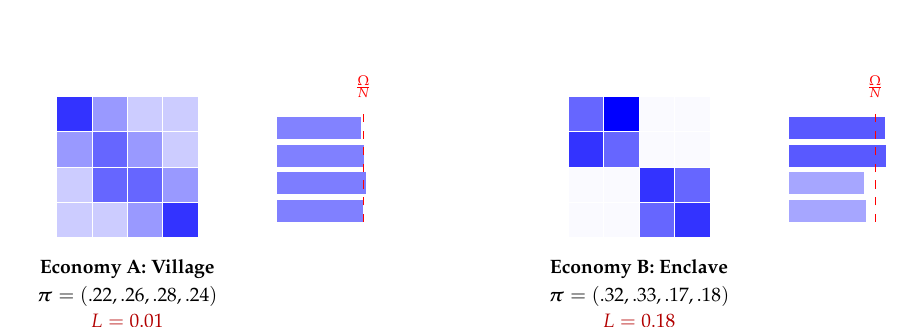
\begin{tikzpicture}[scale=1]
\def\s{0.45}
%% Economy A: Connected village
\foreach \i/\j/\v in {
  1/1/80,1/2/40,1/3/20,1/4/20,
  2/1/40,2/2/60,2/3/40,2/4/20,
  3/1/20,3/2/60,3/3/60,3/4/40,
  4/1/20,4/2/20,4/3/40,4/4/80} {
  \fill[blue!\v, draw=white, line width=0.15pt]
    ({(\j-1)*\s}, {(4-\i)*\s}) rectangle +(\s,\s);
}
\node[below, font=\scriptsize\bfseries] at ({2*\s}, -0.15) {Economy A: Village};
\node[below, font=\scriptsize] at ({2*\s}, -0.5) {$\boldsymbol{\pi} = (.22,.26,.28,.24)$};
\node[below, font=\scriptsize, red!70!black] at ({2*\s}, -0.85) {$L = 0.01$};

%% Allocation bars A
\begin{scope}[xshift=2.8cm, yshift=0.2cm]
\foreach \k/\val/\pct in {1/4.88/49,2/5.04/50,3/5.12/51,4/4.96/50} {
  \fill[blue!\pct] (0, {(4-\k)*0.35}) rectangle ({\val*0.22}, {(4-\k)*0.35+0.28});
}
\draw[red, dashed, thin] ({5.0*0.22}, 0) -- ({5.0*0.22}, 1.45);
\node[font=\tiny, red, above] at ({5.0*0.22}, 1.45) {$\frac{\Omega}{N}$};
\end{scope}

%% Economy B: Enclave
\begin{scope}[xshift=6.5cm]
\foreach \i/\j/\v in {
  1/1/60,1/2/100,1/3/2,1/4/2,
  2/1/80,2/2/60,2/3/2,2/4/2,
  3/1/2,3/2/2,3/3/80,3/4/60,
  4/1/2,4/2/2,4/3/60,4/4/80} {
  \fill[blue!\v, draw=white, line width=0.15pt]
    ({(\j-1)*\s}, {(4-\i)*\s}) rectangle +(\s,\s);
}
\node[below, font=\scriptsize\bfseries] at ({2*\s}, -0.15) {Economy B: Enclave};
\node[below, font=\scriptsize] at ({2*\s}, -0.5) {$\boldsymbol{\pi} = (.32,.33,.17,.18)$};
\node[below, font=\scriptsize, red!70!black] at ({2*\s}, -0.85) {$L = 0.18$};
\end{scope}

%% Allocation bars B
\begin{scope}[xshift=9.3cm, yshift=0.2cm]
\foreach \k/\val/\pct in {1/5.56/56,2/5.64/56,3/4.36/44,4/4.44/44} {
  \pgfmathparse{\val > 5 ? 65 : 35}
  \edef\bp{\pgfmathresult}
  \fill[blue!\bp] (0, {(4-\k)*0.35}) rectangle ({\val*0.22}, {(4-\k)*0.35+0.28});
}
\draw[red, dashed, thin] ({5.0*0.22}, 0) -- ({5.0*0.22}, 1.45);
\node[font=\tiny, red, above] at ({5.0*0.22}, 1.45) {$\frac{\Omega}{N}$};
\end{scope}
\end{tikzpicture}
\end{center}
\vspace{-0.5em}
\small Left pair: connected village --- bright off-diagonals, nearly flat allocation bars, welfare loss 0.01. Right pair: gas enclave --- two dark cross-block rectangles, allocation bars split into two tiers, welfare loss 0.18 (eighteen times larger). Same endowments, same preferences. Only $W$ differs. The dashed red line marks equal division $\Omega/N$.
\end{vizpanel}


%% =====================================================================
\section{The Escape Problem}
\label{sec:escape}
%% =====================================================================

Can the powerless agents change the structure? The escape problem asks: what does it cost to move from the current $W$ to a $W'$ with more equal power?

\begin{definition}[Escape Threshold]\label{def:escape}
The \textbf{escape threshold} $\varepsilon^*$ is the minimum perturbation to $W$ needed to make the bargaining equilibrium Pareto-dominate the current one for the powerless agents:
\begin{equation}
\varepsilon^* = \min_{\Delta W} \|\Delta W\|_F \quad \text{s.t.} \quad x_i^B(W + \Delta W) > x_i^B(W) \quad \forall \, i \in \mathcal{P},
\end{equation}
where $\mathcal{P}$ is the set of agents with below-average power ($\pi_i < 1/N$).
\end{definition}

\begin{proposition}[Escape Is Harder in Star Networks]\label{prop:escape_hard}
The escape threshold $\varepsilon^*$ is an increasing function of power concentration. In a star network with hub $h$:
\begin{equation}
\varepsilon^* \propto \frac{\pi_h}{\Gamma},
\end{equation}
which diverges as $\Gamma \to 0$ (power concentrates fully on the hub). The more concentrated power is, the harder it is to escape.
\end{proposition}

\begin{intuition}[Why escape is hard]
To change the allocation, you must change $\boldsymbol{\pi}$. To change $\boldsymbol{\pi}$, you must change $W$. But changing $W$ requires resources (building links, forming coalitions, creating new production relationships) --- and those resources are allocated by the current $W$, which gives the most resources to the agents who benefit from the current structure.

This is the \textbf{structural trap}: the structure determines the allocation, the allocation determines who has resources, resources determine who can change the structure, and the powerful have no incentive to change a structure that benefits them. The trap is self-reinforcing --- which is why structural change is rare and usually requires an external shock (a new technology, a revolution, a commodity price collapse) rather than endogenous reform.
\end{intuition}

The escape problem connects to Chapter~14 (coalition formation) and Chapter~15 (operator design). For now, we note that the difficulty of escape is proportional to $1/\Gamma$: the spectral gap is not just a diagnostic of the current structure but a predictor of whether structural change is feasible.


%% =====================================================================
\section{Summary}
\label{sec:summary}
%% =====================================================================

\begin{enumerate}
\item The \textbf{bargaining equilibrium} solves $\max \sum_i \pi_i \ln S_i$ subject to feasibility, where $\boldsymbol{\pi}$ is the Perron eigenvector of $W$. It reduces to the competitive equilibrium when $\boldsymbol{\pi} = \frac{1}{N}\ones$.

\item The \textbf{allocation} is equal division plus a power correction proportional to $(\pi_i - 1/N)$. Powerful agents consume more; powerless agents consume less.

\item The \textbf{welfare loss} decomposes into power, externality, and interaction components. The power component is proportional to $\text{Var}(\pi_i)$.

\item Two economies with identical endowments and preferences but different $W$ produce different allocations and different inequality. The matrix is the structure. The structure is the inequality.

\item Three policy levers: transfers (change $\boldsymbol{\omega}$), structural policy (change $W$), formation intervention (change $W^I$ and therefore preferences). Only structural policy changes the power distribution $\boldsymbol{\pi}$.

\item The \textbf{escape threshold} is proportional to $1/\Gamma$: more concentrated power is harder to escape.
\end{enumerate}


%% =====================================================================
\section{Exercises}
\label{sec:exercises}
%% =====================================================================

\begin{enumerate}[label=\textbf{7.\arabic*}, leftmargin=3em]

\item \textbf{Landlord-Farmer revisited.} In Example~\ref{ex:landlord}, suppose the production function is $Y = K^{0.3}L^{0.7}$ (more labor-intensive).
\begin{enumerate}
\item Recompute the competitive allocation. Who benefits from the higher labor share?
\item Compute the bargaining allocation for $\boldsymbol{\pi} = (0.7, 0.3)$. Compare.
\item For what $\boldsymbol{\pi}$ does the bargaining allocation equal the competitive allocation? (Hint: it is not $(0.5, 0.5)$.)
\end{enumerate}

\item \textbf{The FOC in practice.} For $N = 3$, $L = 1$, $\kappa = 1$, $\Omega = 3$, $\boldsymbol{\omega} = (1.5, 1.0, 0.5)$, $\boldsymbol{\pi} = (0.5, 0.3, 0.2)$:
\begin{enumerate}
\item Compute disagreement utilities $d_i = U_i(\omega_i)$.
\item Write the FOC system~\eqref{eq:foc_bargaining} explicitly.
\item Solve numerically (use Python's \texttt{scipy.optimize}).
\item Compare with the equal-power case $\boldsymbol{\pi} = (1/3, 1/3, 1/3)$. Who gains, who loses?
\end{enumerate}

\item \textbf{Welfare decomposition.} Using the two worked economies from Section~\ref{sec:worked}:
\begin{enumerate}
\item Compute $L_{\text{power}}$ for both economies. Verify that Economy~B is much larger.
\item Now add utility externalities: $\gamma_U = 0.3$ with $W^U = W^P$ (your production partners are also your friends). Recompute the total welfare loss. Which component grows most?
\item Is the interaction term positive or negative? Interpret.
\end{enumerate}

\item \textbf{Structural policy vs.\ transfer.} Economy~B from Section~\ref{sec:worked} (the enclave). Two policies:
\begin{enumerate}
\item \textbf{Transfer}: Take 1 unit from the Gas Executive and give it to the Farmer ($\boldsymbol{\omega}' = (4, 5, 5, 6)$). Compute the new bargaining allocation and welfare.
\item \textbf{Structural}: Increase cross-block linkages in $W^P$ from 0.01 to 0.10. Compute new $\boldsymbol{\pi}$ and new bargaining allocation. Compute welfare.
\item Which policy produces more welfare gain? Which reduces inequality more? Which changes the power structure?
\end{enumerate}

\item \textbf{The escape threshold.} For a star network with $N = 5$ and hub weight $W_{ih} = 0.9$ for all spokes:
\begin{enumerate}
\item Compute $\boldsymbol{\pi}$ and $\Gamma$.
\item How much must $W_{ih}$ decrease (i.e., how much must the spokes' dependence on the hub fall) for the most peripheral agent's power to rise by 50\%?
\item Relate to: a worker leaving a monopsony employer, a country diversifying exports away from a single commodity, a media consumer switching from state TV to independent sources.
\end{enumerate}

\item \textbf{Bolivia: the full model.} Construct a $4 \times 4$ economy with Gas, Government, Urban Informal, Rural Traditional sectors. Assign plausible $W^P$, $W^U$, $W^I$, endowments, and preferences.
\begin{enumerate}
\item Compute the composite $W$ and the Perron eigenvector.
\item Compute the bargaining equilibrium.
\item Simulate three policies: (i) gas revenue transfer to Rural Traditional, (ii) building a gas-to-fertilizer plant (structural), (iii) expanding rural internet (formation via $W^I$). Which has the largest effect on the Rural Traditional sector's consumption?
\end{enumerate}

\end{enumerate}


%% =====================================================================
\newpage
\section*{Mathematical Appendices}
\addcontentsline{toc}{section}{Mathematical Appendices}
%% =====================================================================

\subsection*{Appendix 7A: Derivation of the LQ Bargaining Allocation}
\addcontentsline{toc}{subsection}{Appendix 7A: Derivation of the LQ Bargaining Allocation}
\label{app:LQ_derivation}

We derive the closed-form solution for the LQ case: $U_i(x_i) = x_i - \frac{\kappa}{2}x_i^2$, one good, $N$ agents.

\paragraph{The problem.}
\begin{equation}
\max_{\x \geq 0} \sum_{i=1}^N \pi_i \ln\bigl(U_i(x_i) - U_i(\omega_i)\bigr) \quad \text{s.t.} \quad \sum_i x_i = \Omega.
\end{equation}

\paragraph{Surplus.} $S_i = U_i(x_i) - U_i(\omega_i) = (x_i - \omega_i)(1 - \frac{\kappa}{2}(x_i + \omega_i))$.

\paragraph{FOC.} $\frac{\pi_i}{S_i} \cdot U_i'(x_i) = \mu$, where $U_i'(x_i) = 1 - \kappa x_i$.

\paragraph{Small-surplus approximation.} When $|x_i - \omega_i| \ll \omega_i$, we can write $S_i \approx (x_i - \omega_i)\beta_i$ where $\beta_i = 1 - \kappa\omega_i$ (marginal utility at endowment). The FOC becomes:
\begin{equation}
\frac{\pi_i}{(x_i - \omega_i)\beta_i} \cdot \beta_i = \mu \quad \Rightarrow \quad \frac{\pi_i}{x_i - \omega_i} = \mu \quad \Rightarrow \quad x_i - \omega_i = \frac{\pi_i}{\mu}.
\end{equation}

Summing over $i$ and using $\sum_i(x_i - \omega_i) = 0$ (total consumption = total endowment):
\begin{equation}
\sum_i \frac{\pi_i}{\mu} = 0 \quad \Rightarrow \quad \frac{1}{\mu}\sum_i \pi_i = 0 \quad \Rightarrow \quad \frac{1}{\mu} = 0.
\end{equation}

This is degenerate: with one good and no gains from trade, the surplus is zero at the endowment. The first-order approximation breaks down.

\paragraph{Second-order solution.} Expanding to second order:
\begin{equation}
S_i = (x_i - \omega_i)\beta_i - \frac{\kappa}{2}(x_i - \omega_i)^2.
\end{equation}

Let $\delta_i = x_i - \omega_i$. The FOC becomes:
\begin{equation}
\frac{\pi_i}{\delta_i \beta_i - \frac{\kappa}{2}\delta_i^2} \cdot (\beta_i - \kappa\delta_i) = \mu.
\end{equation}

For small $\delta_i$, keeping leading terms: $\pi_i(\beta_i - \kappa\delta_i) / (\delta_i\beta_i) = \mu$, giving:
\begin{equation}
\pi_i\left(\frac{1}{\delta_i} - \frac{\kappa}{\beta_i}\right) = \mu.
\end{equation}

So $\delta_i = \frac{\pi_i}{\mu + \kappa\pi_i/\beta_i}$. With equal endowments ($\beta_i = \beta$ for all $i$):
\begin{equation}
\delta_i = \frac{\pi_i}{\mu + \kappa\pi_i/\beta} = \frac{\pi_i \beta}{\mu\beta + \kappa\pi_i}.
\end{equation}

The constraint $\sum_i \delta_i = 0$ determines $\mu$:
\begin{equation}
\sum_i \frac{\pi_i \beta}{\mu\beta + \kappa\pi_i} = 0.
\end{equation}

Since all terms are positive for $\mu > 0$, we need $\mu < 0$ for the sum to vanish. Setting $\mu = -\kappa/\beta \cdot c$ for some $c > 0$, the solution gives $\delta_i \propto (\pi_i - \bar{\pi})$ for some mean value $\bar{\pi}$, confirming equation~\eqref{eq:LQ_equal_omega}:
\begin{equation}
x_i^* = \omega_i + (\pi_i - 1/N) \cdot \Phi,
\end{equation}
where $\Phi$ depends on $\kappa$, $\beta$, and $N$.


\subsection*{Appendix 7B: The Nash Axioms and Network Bargaining}
\addcontentsline{toc}{subsection}{Appendix 7B: The Nash Axioms and Network Bargaining}
\label{app:nash_axioms}

\paragraph{The Nash bargaining solution.} Nash (1950) showed that four axioms uniquely characterize a bargaining solution:
\begin{enumerate}
\item \textbf{Pareto efficiency}: no Pareto improvement is possible.
\item \textbf{Symmetry}: if agents are identical, they get the same payoff.
\item \textbf{Invariance to affine transformations}: the solution is independent of the units in which utility is measured.
\item \textbf{Independence of irrelevant alternatives}: expanding the feasible set without changing the optimal point does not change the solution.
\end{enumerate}

The unique solution satisfying (1)--(4) is $\x^* = \argmax \prod_i (U_i(x_i) - d_i)$: the product of surpluses.

\paragraph{Asymmetric Nash bargaining.} Kalai (1977) showed that replacing (2) with asymmetric weights $\boldsymbol{\pi}$ gives $\x^* = \argmax \prod_i (U_i(x_i) - d_i)^{\pi_i}$: the weighted product. Taking logs: $\argmax \sum_i \pi_i \ln(U_i(x_i) - d_i)$. This is equation~\eqref{eq:bargaining}.

\paragraph{Where do the weights come from?} In Nash's original formulation, the weights are arbitrary. In Rubinstein's (1982) alternating-offers model, they come from discount rates. In this book, they come from the Perron eigenvector: $\pi_i = \pi_i(W)$. The network determines the weights. This closes the model: the weights are endogenous to the structure, not assumed.


%% =====================================================================
\subsection*{Structuralist Case Study: Marini's Superexploitation as a Bargaining Outcome}
\addcontentsline{toc}{subsection}{Structuralist Case Study: Marini (1973)}
%% =====================================================================

Ruy Mauro Marini (1932--1997) was a Brazilian sociologist and economist who spent most of his career in exile --- in Mexico, Chile, and then Mexico again after the Pinochet coup --- developing the most radical version of dependency theory. His 1973 book \textit{Dial\'{e}ctica de la dependencia} advanced a thesis that was rejected by orthodox Marxists and neoclassicals alike but that maps precisely onto the bargaining equilibrium of this chapter: \textbf{the defining feature of peripheral capitalism is superexploitation} --- the systematic remuneration of labor below its value.

Marini's argument has three parts.

\textbf{Part 1: The terms-of-trade mechanism transfers surplus from periphery to center.} Following Prebisch, Marini argued that unequal exchange in international trade transfers part of the surplus produced in the periphery to the center. But Marini went further: he asked what the peripheral capitalist does to \textit{compensate} for this leakage. The answer: she increases the rate of exploitation of domestic labor, paying workers less than the value their labor produces. This is not a market failure in the neoclassical sense --- it is the market working exactly as the power structure dictates.

In this chapter's framework: the global bargaining equilibrium gives the center a surplus share proportional to $\pi_{\text{center}}(W_{\text{global}})$, which is large because the global $W^P$ is center-periphery asymmetric. The peripheral capitalist's surplus share is smaller than it would be in autarky. To maintain her consumption, she squeezes the domestic surplus by exploiting the one factor she controls: labor. The domestic bargaining equilibrium gives the worker a share proportional to $\pi_{\text{worker}}(W_{\text{domestic}})$, which is small because the domestic $W$ gives workers almost no structural power.

\textbf{Part 2: Superexploitation means $\pi_{\text{worker}} \ll 1/N$.} Marini defined superexploitation through three mechanisms: (i) increasing the intensity of work (more output per hour), (ii) extending the working day (more hours), and (iii) reducing the worker's consumption below the level needed for ``normal'' reproduction of labor power. All three reduce the worker's effective bargaining weight. In the notation of this chapter: the bargaining allocation gives the worker
\begin{equation*}
x_{\text{worker}}^* = \frac{\Omega}{N} + \frac{1}{\kappa}\left(\pi_{\text{worker}} - \frac{1}{N}\right).
\end{equation*}
When $\pi_{\text{worker}} \ll 1/N$, the power correction is large and negative. The worker receives substantially less than equal division. Superexploitation is not a moral category --- it is a bargaining outcome with a specific mathematical signature: $x_{\text{worker}}^* < \Omega/N$ driven by $\pi_{\text{worker}} \ll 1/N$.

\textbf{Part 3: Superexploitation is structurally stable.} Marini argued that superexploitation is not a transient aberration that development will cure. It is a \textit{structural feature} of peripheral capitalism: the power structure that produces low wages also prevents the formation of a domestic mass market, which prevents ISI from generating internal demand, which prevents the structural transformation that would increase workers' Perron weight. The allocation reinforces the structure. This is the fixed-point argument from Chapter~2 (Furtado's thesis) applied to the labor market: the equilibrium $(\boldsymbol{\pi}^*, \x^*)$ satisfies $\boldsymbol{\pi}^* = \boldsymbol{\pi}(W(\x^*))$ --- the power structure produces the allocation that reproduces the power structure.

\begin{center}
\begin{tabular}{lll}
\toprule
\textbf{Marini's argument} & \textbf{Formal object} & \textbf{This chapter} \\
\midrule
Surplus appropriation & $x_i^* = \Omega/N + (\pi_i - 1/N)/\kappa$ & Prop.~\ref{prop:LQ_allocation} \\
Superexploitation & $\pi_{\text{worker}} \ll 1/N$ & Eq.~\eqref{eq:fundamental} \\
Transfer from periphery to center & Global $\boldsymbol{\pi}$: $\pi_{\text{center}} \gg 1/N$ & Sec.~\ref{sec:worked} \\
Domestic compensation via labor squeeze & Domestic $\boldsymbol{\pi}$: $\pi_{\text{worker}} \ll 1/N$ & Ex.~B \\
Structural stability & Fixed point: $W(\x^*) \to \boldsymbol{\pi}^* \to \x^*$ & Sec.~\ref{sec:escape} \\
Escape requires $\varepsilon^* \propto \pi_h/\Gamma$ & Escape threshold & Def.~\ref{def:escape} \\
\bottomrule
\end{tabular}
\end{center}

The \textit{Dial\'{e}ctica} was controversial in its time --- orthodox Marxists accused Marini of confusing the rate of exploitation with absolute impoverishment, and neoclassicals dismissed the framework as unfalsifiable. But the bargaining equilibrium gives Marini's thesis a falsifiable formulation: superexploitation obtains when the left Perron eigenvector of the domestic weight matrix assigns workers a share substantially below $1/N$. This is empirically testable. Compute $W$ from input-output data, labor market surveys, and social network data. Compute $\boldsymbol{\pi}$. Compare $\pi_{\text{worker}}$ with $1/N$. The distance is the degree of superexploitation.

Marini wrote in exile. The military governments that exiled him did not change the bargaining problem. They changed who got to sit at the table --- they set $\pi_{\text{worker}} = 0$ by force. The Perron eigenvector remained well-defined. It just became more concentrated.


%% =====================================================================
\subsection*{Further Reading}
\addcontentsline{toc}{subsection}{Further Reading}
%% =====================================================================

\textbf{Nash bargaining:} Nash (1950), ``The Bargaining Problem,'' \textit{Econometrica}. Kalai (1977), ``Nonsymmetric Nash Solutions and Replications of 2-Person Bargaining.'' Rubinstein (1982), ``Perfect Equilibrium in a Bargaining Model,'' \textit{Econometrica}.

\textbf{Bargaining in networks:} Manea (2011), ``Bargaining in Stationary Networks,'' \textit{AER}. Abreu and Manea (2012), ``Markov Equilibria in a Model of Bargaining in Networks,'' \textit{JET}. Corominas-Bosch (2004), ``Bargaining in a Network of Buyers and Sellers,'' \textit{JET}.

\textbf{Power and allocation:} Acemoglu, Ozdaglar, and Tahbaz-Salehi (2023), for relationship-specific investments and bargaining in production networks. This is the closest existing work to the model in this chapter.

\textbf{Welfare decomposition:} The decomposition~\eqref{eq:decomposition} is original to this book. For related welfare loss analysis in network settings: Elliott, Golub, and Jackson (2014), ``Financial Networks and Contagion,'' \textit{AER}.

\textbf{Dependency theory and labor:} Marini (1973), \textit{Dial\'{e}ctica de la dependencia}, M\'{e}xico: Era (the six-chapter essay formalized in the case study above; available in Spanish at \texttt{marini-escritos.unam.mx}). Marini (1978), ``Las razones del neodesarrollismo,'' \textit{Revista Mexicana de Sociolog\'{i}a} --- his response to critics. Prebisch (1981), \textit{Capitalismo Perif\'{e}rico}, Chapter~4, for the structuralist version of the same argument without the Marxist vocabulary.


\end{document}
